\documentclass[a4paper, 12pt, titlepage]{article}
\usepackage[utf8]{inputenc}
\usepackage{geometry}
\usepackage{polski}
\usepackage{graphicx}
\usepackage{float}
\usepackage{etoolbox,refcount}
\usepackage{multicol}
\usepackage{fancyhdr}
\pagestyle{fancy}
\title{Prototypowanie serwomechanizmu dla zespołu napędowego.}
\author{Adrian Jałoszewski, Tomasz Kotowski}
\date{}
\newgeometry{left=2.5cm, right=2.5cm, bottom=2.5cm, top=2.5cm}

\begin{document}
	\maketitle
	\section{Cel ćwiczenia}
	\section{Wykonanie modelu w Simulinku}
		\begin{figure}[H]
			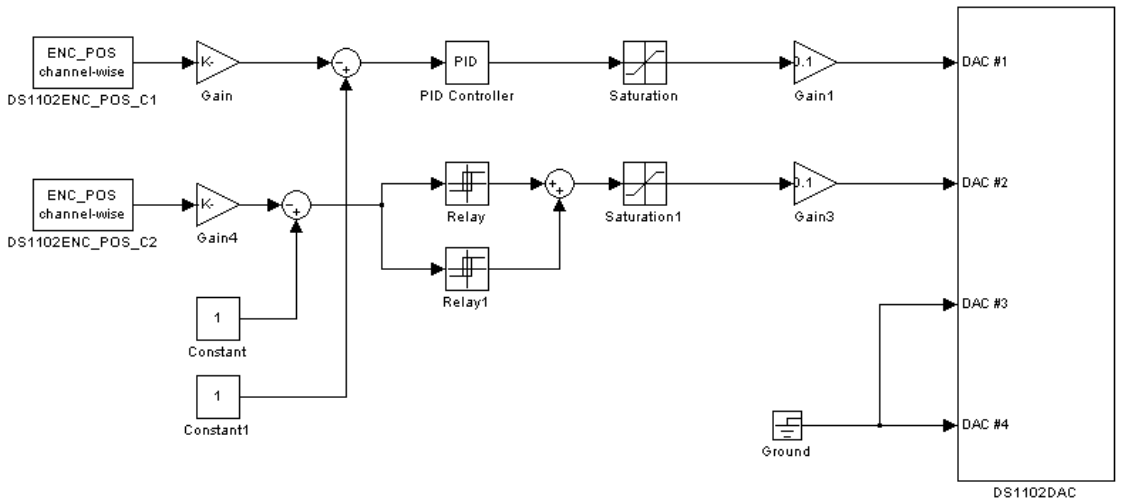
\includegraphics[width=\textwidth]{img/original_system.png}
			\caption{Oryginalny model}
		\end{figure}
		\begin{figure}[H]
			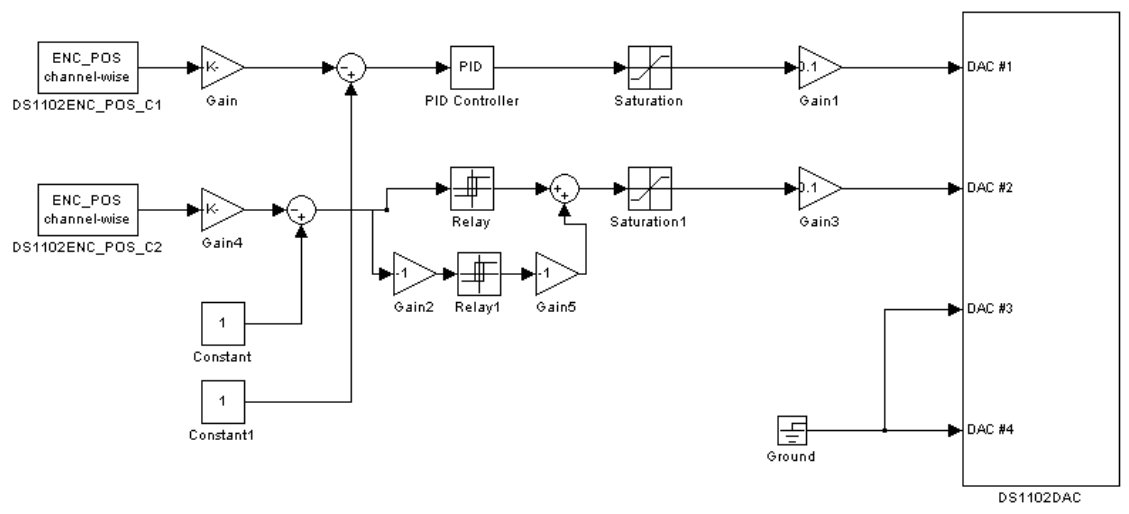
\includegraphics[width=\textwidth]{img/our_improved_system.png}
			\caption{Model z naszymi ulepszeniami}
		\end{figure}
	\section{Wykonanie panelu operatorskiego}
		\begin{figure}[H]
			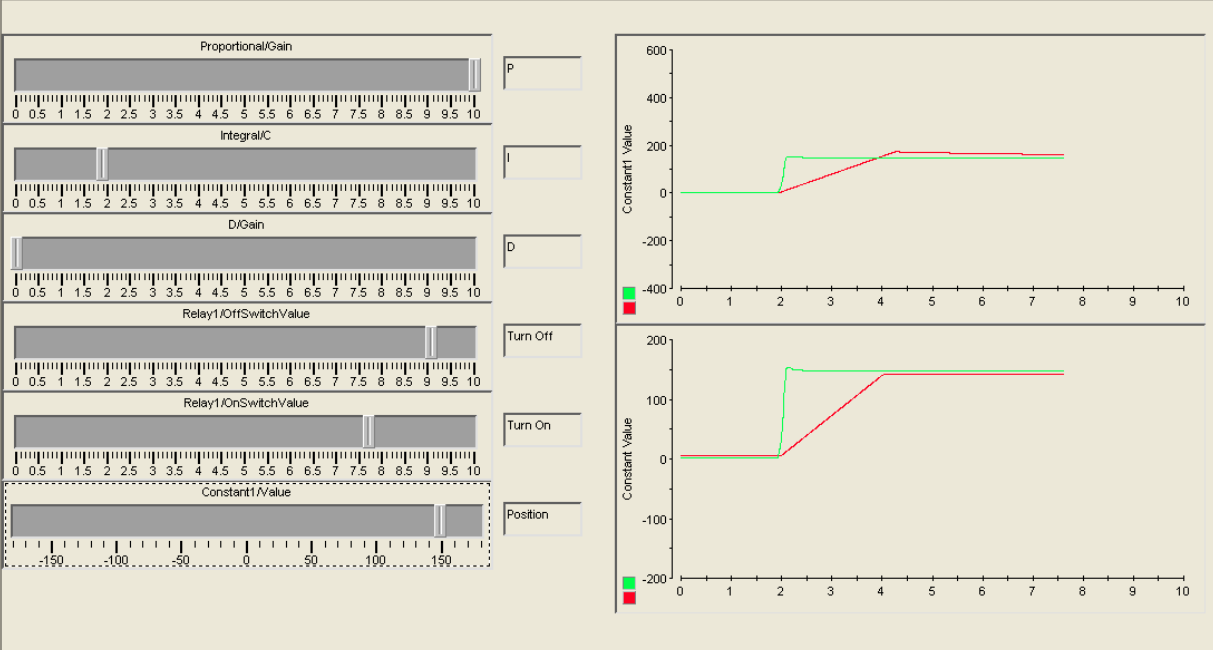
\includegraphics[width=\textwidth]{img/operational_panel.png}
			\caption{Panel operatorski}
		\end{figure}
\end{document}